% Options for packages loaded elsewhere
\PassOptionsToPackage{unicode}{hyperref}
\PassOptionsToPackage{hyphens}{url}
%
\documentclass[
]{article}
\usepackage{amsmath,amssymb}
\usepackage{lmodern}
\usepackage{iftex}
\ifPDFTeX
  \usepackage[T1]{fontenc}
  \usepackage[utf8]{inputenc}
  \usepackage{textcomp} % provide euro and other symbols
\else % if luatex or xetex
  \usepackage{unicode-math}
  \defaultfontfeatures{Scale=MatchLowercase}
  \defaultfontfeatures[\rmfamily]{Ligatures=TeX,Scale=1}
\fi
% Use upquote if available, for straight quotes in verbatim environments
\IfFileExists{upquote.sty}{\usepackage{upquote}}{}
\IfFileExists{microtype.sty}{% use microtype if available
  \usepackage[]{microtype}
  \UseMicrotypeSet[protrusion]{basicmath} % disable protrusion for tt fonts
}{}
\makeatletter
\@ifundefined{KOMAClassName}{% if non-KOMA class
  \IfFileExists{parskip.sty}{%
    \usepackage{parskip}
  }{% else
    \setlength{\parindent}{0pt}
    \setlength{\parskip}{6pt plus 2pt minus 1pt}}
}{% if KOMA class
  \KOMAoptions{parskip=half}}
\makeatother
\usepackage{xcolor}
\usepackage{longtable,booktabs,array}
\usepackage{multirow}
\usepackage{calc} % for calculating minipage widths
% Correct order of tables after \paragraph or \subparagraph
\usepackage{etoolbox}
\makeatletter
\patchcmd\longtable{\par}{\if@noskipsec\mbox{}\fi\par}{}{}
\makeatother
% Allow footnotes in longtable head/foot
\IfFileExists{footnotehyper.sty}{\usepackage{footnotehyper}}{\usepackage{footnote}}
\makesavenoteenv{longtable}
\setlength{\emergencystretch}{3em} % prevent overfull lines
\providecommand{\tightlist}{%
  \setlength{\itemsep}{0pt}\setlength{\parskip}{0pt}}
\setcounter{secnumdepth}{3} % enable section numbering
\ifLuaTeX
  \usepackage{selnolig}  % disable illegal ligatures
\fi
\IfFileExists{bookmark.sty}{\usepackage{bookmark}}{\usepackage{hyperref}}
\IfFileExists{xurl.sty}{\usepackage{xurl}}{} % add URL line breaks if available
\urlstyle{same} % disable monospaced font for URLs
\usepackage{csquotes}
\usepackage[style=apa,sortcites=true,sorting=nyt,backend=biber]{biblatex}
\DeclareLanguageMapping{american}{american-apa}
\addbibresource{MyBib.bib}
\usepackage{listings}
\usepackage{enumitem}
\usepackage{float}
\usepackage{graphicx}
\hypersetup{
  hidelinks,
  pdfcreator={LaTeX via pandoc}}

\author{}
\date{}

\begin{document}

\textbf{Enhancing Data Labels using Large Language Models for Bilingual
Malay-English Hate Speech Detection\\
}Jordan Ling Shen Hang¹, Sook-Ling Chua¹\textsuperscript{,*}, Lee
Kien Foo¹

\emph{¹ Faculty of Computing and Informatics, Multimedia University,
Cyberjaya, Malaysia}

\emph{\{jordan.ling.shen, slchua, lkfoo\}@mmu.edu.my}

\textbf{Abstract.} With the rise of social networking the spread and volume of fake news has dramatically increased, to the point where fact checking every post is unrealistic. In attempts to solve this problem, researchers have proposed methods employing machine learning and deep learning to flag fake news. However, these methods are often limited by lack of applicability as they fail to generalise beyond the datasets used. Furthermore, many of these methods employ black-box models, which reduces trust in the model's predictions. In order to address these issues, we proposed a model based on adversarially fine-tuning a Bidirectional Encoder Representations from Transformers (BERT) model to increase generalisation, and the use of Local Interpretable Model-Agnostic Explanations (LIME) to explain the otherwise black-box BERT model. Results indicated that while this technique failed to effectively generalise the model, the LIME implementation was successful and highlighted the reasons for the model's output.

\textbf{Keywords:} 

\section{Introduction}

Fake news threatens personal, organisational and institutions by creating distrust and damaging reputations. Fake news can be particularly damaging as even if it can be refuted, it may still cause lasting damage to reputations. With the widespread use of social media, the proliferation of fake news has greatly increased both in terms of speed and quantity. This has led to the sheer volume of fake news (and real news) overwhelming human fact-checkers and preventing them from manually verifying all content. 

But what is fake news? According to \textcite{definition} the definition of fake news is generally agreed to be either completely or partially false information, with varying levels of agreement for other additional criteria. Such as the intent to deceive, and if only content in a news format should be counted. For the purpose of this research, the working definition of fake news defined by \textcite{definition} will be used: 

\begin{quote}
    a type of online disinformation (1), with (2) misleading
and/or false statements that may or may not be associated with real events, (3) intentionally
created to mislead and/or manipulate a public (4) specific or imagined, (5) through the
appearance of a news format with an opportunistic structure (title, image, content) to attract
the reader’s attention, in order to obtain more clicks and shares and, therefore, greater
advertising revenue and/or ideological gain \textcite{definition}
\end{quote} 

In a recent (as of writing) example of fake news causing adverse impact, \textcite{Savage-Guardian_2025} wrote for The Guardian about YouTube channels spreading fake news about UK politics in their videos, accruing close to 1.2 billion views in total. While some forms of news which are factually fake are usually harmless (parody, satire, etc.) fake news, with the intent or deceiving those who consume it is dangerous, it can widen division, spread prejudice and cause distrust in institutions are among just a few examples. And while fake news may sound innocuous enough, 'It's just fake news, ignore it', it can lead to serious consequences, including injury and death. In one such example, during the COVID-19 vaccination campaign in Taiwan an adverse correlation between prevalence of fake news and vaccination rates were found \parencite{vaccination}.

As a result, the development of automated fake news detection systems have been explored. But limitations related to generalisation where detection systems perform poorly on data which did not appear in its training sets \parencite{BERT-finetuning} limit their applicability. Additionally, current methods such as Machine Learning (ML) approaches, fail to capture the semantic data meaningfully, reducing its detection accuracy. Furthermore, many approaches which employ Deep Learning (DL) are often black-boxes, which results in lowered trust towards these systems \parencite{xai-bert}. 

This highlights the need for new approaches which are capable of detecting fake news by analysing the semantic information in the text thoroughly, having greater generalisation and be more transparent (explainable) when making its classifications.

\section{Literature Review}

An issue with current models is that while they work well with data which was found in their training sets, they often suffer in performance when they encounter data unknown to them \parencite{BERT-finetuning}. To solve this issue, \textcite{BERT-finetuning} proposed a novel approach, Feature Regularization-based Adversarial Fine-tuning (FGM-FRAT). This approach generates perturbed versions of the input in order to confuse the model. This forces the model to find new, deeper patterns instead of relying on otherwise superficial features. The key innovation however, is the addition of a regularization term to the loss function which seeks to minimise the difference between the features generated from the unperturbed, original text with the features generated from the perturbed text. This ensures the feature representation generated by the model will remain similar between original and perturbed text, improving generalisation. The authors used the FakeNewsNet dataset to fine-tune a BERT model using the FGM-FRAT approach using the FakeNewsNet dataset. The authors then tested the fine-tuned model with unseen datasets (BuzzFeedNews, LIAR, WELFake and KaggleFakeNews), using the standard BERT model as a baseline as well as some other fine-tuned BERT models which were fine-tuned with various approaches. The BERT-FGM-FRAT model performed the best amongst all models tested, with improvements of up to 0.32 in terms of F1-score against the base BERT model on the BuzzFeedNews dataset. While for other datasets the BERT-FGM-FRAT managed to offer significant performance improvements with the sole exception of the WELFake dataset where it was only able to improve upon the base model incrementally with a 0.03 (F1-score) improvement. 

\textcite{gbert} proposed a new deep learning model for predicting fake news called "Generative Bidirectional Encoder Representations from Transformers" or GBERT, a hybrid of Generative Pre-Trained Transformer (GPT) and Bidirection Encoder Representations from Transformers (BERT). The authors used two benchmark Indian datasets: The Indian Fake News Dataset (IFND) and FakeNewsIndia Dataset. The standard cleaning and normalisation of the textual data was applied including: decapitalisation, removal of URLs, names, punctuation stop words, numbers and emojis, and the application of stemming and lemmitisation. Now for the feature extraction the cleaned data is fed into two Large Language Model (LLM) components, BERT and GPT. BERT captures word embeddings, with context from every token input into it and outputs a summary of the context inside the input sequence. While GPT captures the global dependencies and semantic coherence in the input data and outputs the last hidden state of the final token. Finally the output from BERT and GPT (the features) are merged together in a concatenation layer before being passed to the dense layer for the final binary classification using a Sigmoid function. The results showed that the proposed GBERT model performed well, with a F1-score of 0.9623. It is worth noting, however, that XGBoost performed well in terms of accuracy (F1-score was not provided for XGBoost) with a score of 93.42\% while the proposed GBERT model has a score of 95.30\%.

Research by \textcite{xai-bert} proposed a novel approach which sought to make the model's decision-making explainable (explainable AI), the reason being that having a black-box system determine the veracity of something doesn't inspire confidence, something an explainable AI model could mitigate. The researchers utilised DistilBERT which is a lighter variant of BERT, combined with an LSTM layer, a pooling layer, dense feed forward layer and finally the output layer. They then attached an explainability module to the black-box classifier. This module is composed of two post-hoc explainable AI techniques, Local Interpretable Model-Agnostic Explanations (LIME) and Anchors. Post-hoc refers to techniques which attempt to give some level of transparency to an otherwise black-box model. LIME works by sampling the model in the vicinity of a prediction (imagine having an unknown 'X' on a spot on a graph and then picking spots around it to approximate the 'X''s coordinates) and the response to the sampling is used to train a linear model that approximates the model's prediction that can be interpreted. While Anchors refer to an algorithm that applies 'rules' to local predictions, the rules being 'if-then' statements which should ensure that any prediction will remain the same wherever the rule holds. The model was able to achieve 0.98 F1-score for both positive and negative classes. The researchers were able to conclude from the results that it is feasible to use methods such as LIME and Anchors to explain the models behaviour. Although there was some overlap between LIME and the Anchors when explaining the model's behaviour, the results showed it is possible to use multiple types of these methods can be used to derive explanations. 

\textcite{Xflag} proposed an explainable AI approach, XFlag, to fake news detection which sought to increase the transparency and trust of black-box AI models. The authors used the Weibo dataset, which was processed to extract content, user and sentiment features. Content features were extracted with Doc2Vec which generates word embeddings from the content, similar to BERT, albeit Doc2Vec is an older model. User features were extracted from the user's profile, such as followers, location, etc.. Sentiment features were extracted with the Google Cloud Natural Language API which returned the emotional, "sentimental" data from the content. These features are then passed to fully connected layers before being passed to the LSTM in order to standardise the input to the LSTM. XFlag was able to perform comparably to state of the art models, with an F1-score of 0.938. As for the explainability, the authors used the Layer-wise Relevance Propagation (LRP) algorithm which uses reverse propagation, essentially start with the model output and going in the reverse direction through the model's various layers to determine which neurons had the most impact on the result. The output of the LRP would be the model's (being tested) input shape but with the relevance score for each neuron, this is known as the explanation vector. LRP was applied to the XFlag model after the model was trained, and the output explanation vectors are then passed to Situation Awareness-based Agent Transparency (SAT) framework, specifically the SAT-3 (the researchers used other SAT versions from SAT 1 - 3 which each iteration having more insightful explanations, SAT-3 was most preferred by users) which takes this raw data and processes it in order to generate visualisations, textual annotations and the model's uncertainty so that the user can see how the model came to the conclusion that it did. Users were tested on their trust of the XFlag model with various SAT versions, the lowest being SAT-1 which, similar to a model with no explainability, output the result without deeper explanation. The results were that users reported highest satisfaction and trust as the SAT level and correspondingly, the depth of the explanations of the model's prediction, increased, the highest being SAT-3. 

\section{Proposed Method}
The proposed model, Text Perturbation-based Adversarial BERT (TPA-BERT), sought to improve the generalisation when it comes to fake news detection, particularly against unseen data. This was to be done by directly perturbing the text, followed by adversarial training to minimise the difference in embeddings generated when given original and perturbed data. The intention is, by scrambling the text, and with the adversarial training minimising the differences in model output, TPA-BERT would generate embeddings which are more robust and learn to identify more 'in-depth' features for fake news detection.

Going in more depth regarding the methodology: firstly, before any training began, the datasets are perturbed using NLTK's WordNet by loading each record and applying synonym substitution against 20\% of each record's words, followed by another 10\% of words which are randomly swapped (swapped between words in the same row) and lastly 10\% of words are randomly deleted. Secondly, the BERT model is loaded, and both the original and perturbed datasets and conducting stratified splits of the data (85\% train, 15\% test) which is followed by a 80\%-20\% train and validation split (on the 85\% train set; remaining 15\% saved for final evaluation)for k=5 cross validation. Following this, the training begins with the model accepting input capped at 128 tokens (per record) and beginning to learn from the adversarial loss function which combines the cross entropy loss and cosine similarity loss (the difference between the CLS tokens produced by the model for the original and perturbed data input). Note that the cosine similarity loss is linearly scaled from 0 to 0.5 over the first 10\% of training steps. Once training is complete, whether by completing all epochs, or by early-stopping (set at 3 steps) the model is evaluated on the held out test set. And to test the model's generalisation, the best model according to validation f1-score is chosen for cross-dataset evaluation (tested against all other datasets; for example: a model trained on WELFake is tested on FakeNewsNet, ISOT, Fake News Classification and Fake News Detection datasets). 

$$\text{Loss} = \text{CE_Loss} + \lambda_{adv} \times \text{Cosine_Similarity_Loss}$$

\begin{lstlisting}[language=Python, caption={BERT Fine-tuning Configuration}]
training_kwargs = {
    "output_dir": f'./results_adv_fold_{fold+1}',
    "num_train_epochs": 3,
    "per_device_train_batch_size": 32,
    "per_device_eval_batch_size": 32,
    "gradient_accumulation_steps": 2,
    "save_strategy": "steps",
    "save_steps": 128,
    "save_total_limit": 1,
    "bf16": use_tpu,
    "gradient_checkpointing": not use_tpu,
    "report_to": "none",
    "optim": "adamw_torch",
    "logging_dir": './logs',
    "logging_steps": 128,
    "metric_for_best_model": "f1",
    "load_best_model_at_end": True,
    "weight_decay": 0.01,
    "remove_unused_columns": False,
    "label_names": ["labels"],
}
\end{lstlisting}
*Note that although eval_steps and eval_strategy are not in the parameter list, by default the strategy is "steps" and the steps are "128".

There are several modifications to the parameters compared to the baseline BERT model. Most notably the training batch size which is now 32 instead of the 128 used by the baseline. There are a few reasons for this: firstly, the model also has to process the adversarial data which essentially doubles the data processed. And secondly, because of the aforementioned doubled data, the forward and backward passes now carry twice as much data. As a result, with double the data as well as the fact the forward and backward passes also have to deal with double the data, the effective batch size is 128. 

The proposed model is inspired by and similar to the process described by \textcite{BERT-finetuning}, however, unlike the model described by those authors, TPA-BERT perturbs the text directly, instead of at the embedding and feature level like in FGM-FRAT (the model described by the authors). The reason for this deviation is that perturbation at a text level is simple to implement, in addition to the decreased number of passes per step thus reducing computational demands. Furthermore, the proposed model also contains a LIME component which will complement the BERT component by giving explanations for the otherwise black box model to increase trust in the model. 

\section{Methodology}

\subsection{Datasets}
\subsubsection{WELFake Dataset}
The WELFake dataset was downloaded from Kaggle, and contains 72134 rows of data. The class balance was relatively balanced, with the real news class having an excess of 2000 rows as can be referred to in Figure \ref{fig:welfake_dist}. As for features, the dataset came with four columns, an unnamed ID column, title (of the news article), text (from the news article) and the label (real/fake). There were 558 missing values in the 'title' column and 39 missing values in the 'text' column initially.

\begin{figure} [H]
    \centering
    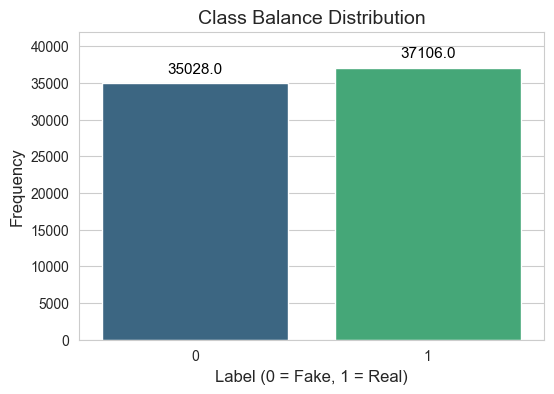
\includegraphics[width=0.5\linewidth]{WELFake class distribution.png}
    \caption{Figure depicts the class distribution of the WELFake dataset}
    \label{fig:welfake_dist}
\end{figure}

\subsubsection{Fake News Classification}
This dataset, named "Fake News Classification" was downloaded from Kaggle. It contains 40597 rows of data with 4 columns: an unnamed ID column, title, text and label. There were no missing values or duplicates in any of the rows initially before pre-processing. And the class balance had an excess of approximately 3000 in favour of the positive class (real). 

\begin{figure} [H]
    \centering
    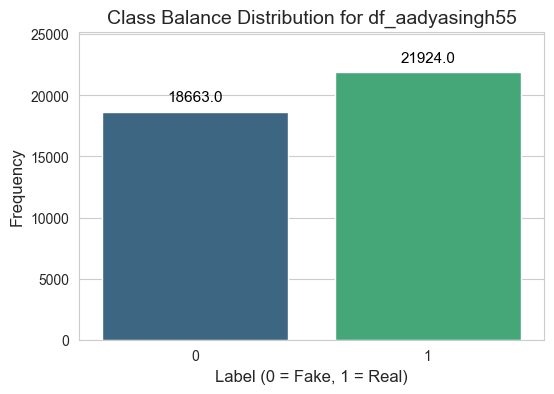
\includegraphics[width=0.5\linewidth]{Fake news classification class balance.png}
    \caption{Figure depicts the class distribution of the Fake News Classification dataset}
    \label{fig:fake_news_class_dist}
\end{figure}

\subsubsection{FakeNewsNet}
The FakeNewsNet dataset was downloaded from Kaggle, it is worth noting this was not the original dataset, it had its various Comma Separated Values (CSV) files merged by the uploading user "algord". The original dataset was gathered and used for research by \textcite{shu2018fakenewsnet}, \textcite{shu2017exploiting} and \textcite{shu2017fake}. We thank the authors for developing and providing this dataset for use. FakeNewsNet contains 23196 rows, with 5 columns: title, news\_url, source\_domain, tweet\_num and label. The dataset contained missing values in the news\_url and source\_domain columns (which is acceptable as this is not required later on in training or testing). There were 137 duplicate rows (which will be dropped later on) initially. The class balance was heavily skewed in favour of the positive (real) class, with approximately 75\% of all rows belonging to the positive class. 

\begin{figure} [H]
    \centering
    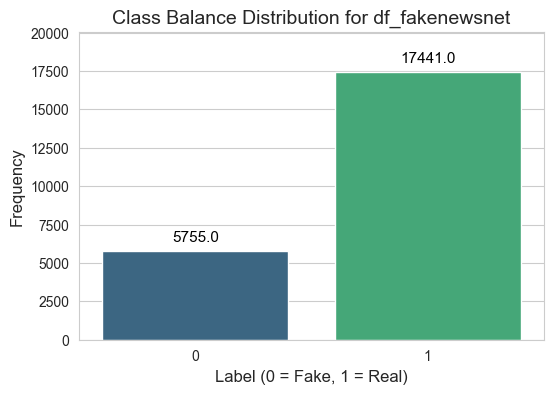
\includegraphics[width=0.5\linewidth]{FakeNewsNet class distribution.png}
    \caption{Figure depicts the class distribution of the FakeNewsNet dataset}
    \label{fig:fakenewsnet_dist}
\end{figure}

\subsubsection{Fake News Detection}
The Fake News Detection dataset was downloaded from Hugging Face. It contains 44267 rows and 6 columns: Unnamed ID column, title, text, subject, date, and label. There were no missing values or duplicate rows initially. The class balance is relatively balanced with the difference between the positive and negative classes being approximately ± 3\%. 

\begin{figure} [H]
    \centering
    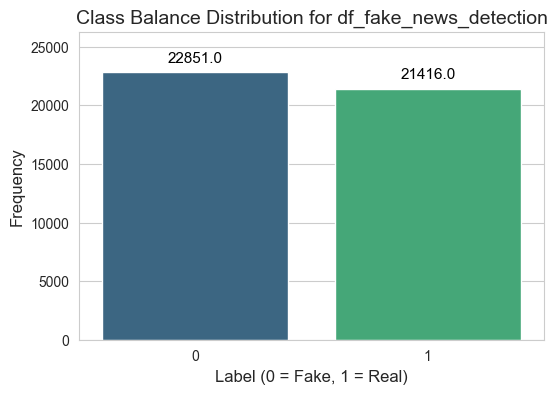
\includegraphics[width=0.5\linewidth]{fake news detection class balance.png}
    \caption{Figure depicts the class distribution of the Fake News Detection dataset}
    \label{fig:fake_news_detection_dist}
\end{figure}

\subsubsection{ISOT}
The ISOT dataset was downloaded from the University of Victoria website. It was originally gathered and used for research by \textcite{isot1} and \textcite{isot2}. We thank the authors for gathering this dataset and providing it. It contains 44898 rows with 5 columns: title, text, subject, date and label. There were no missing values initially. However, there were 209 duplicate rows initially. The class balance was relatively balanced, with the difference in proportion of the positive and negative classes being approximately ± 5\%.

\begin{figure} [H]
    \centering
    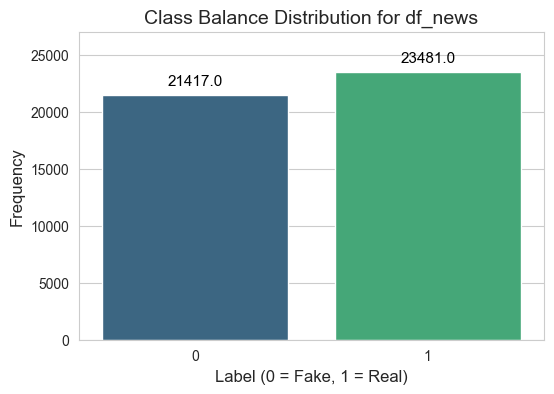
\includegraphics[width=0.5\linewidth]{ISOT class balance.png}
    \caption{Figure depicts the class distribution of the ISOT dataset}
    \label{fig:isot_dist}
\end{figure}


\subsection{Data Preprocessing}
The data was processed by first merging 'title' and 'text' columns together if the dataset had split 'title' and 'text' into different columns, this would be combined. In one of the datasets "FakeNewsNet", only the 'title; column was used. After the columns were combined, the new 'combined\_text' column was checked for missing strings and null values, of which none were found.

After combining the columns, any columns that did not contain the label or 'combined\_text' column were dropped, such as source URLs columns, and other metadata like date. This revealed substantially more duplicated rows, likely as a result of the datasets being gathered through scraping methods which scraped the same content from multiple sources causing the dataset to have duplicated textual columns but different metadata, which allowed it to evade detection earlier. The total number of samples dropped is summarised in Table \ref{tab:preprocessing_stats}.

Once completed, the 'combined\_text' column was stripped of any non-Unicode characters as well as links, phone numbers and other non-ASCII characters. The removal of non-ASCII characters is possible as this research focuses on English news. After this, any rows with empty strings are removed. 

\begin{table}[H]
    \centering
    \scriptsize % Reduces font size slightly to fit width
    \setlength{\tabcolsep}{3pt} % Reduces space between columns
    \caption{Summary of Data Preprocessing Statistics}
    \label{tab:preprocessing_stats}
    \begin{tabular}{l cc cc cc cc}
        \toprule
         & \multicolumn{2}{c}{\textbf{Initial}} 
         & \multicolumn{2}{c}{\textbf{After Combining Text}} 
         & \multicolumn{2}{c}{\textbf{After Dropping Rows}} 
         & \multicolumn{2}{c}{\textbf{After Cleaning}} \\
        \cmidrule(lr){2-3} \cmidrule(lr){4-5} \cmidrule(lr){6-7} \cmidrule(lr){8-9}
        \textbf{Dataset} & \textbf{Missing*} & \textbf{Duplicates} & \textbf{Missing*} & \textbf{Duplicates} & \textbf{Missing*} & \textbf{Duplicates} & \textbf{Missing*} & \textbf{Duplicates} \\
        \midrule
        WELFake & 597 & 0 & 0 & - & - & 8458 & 6 & - \\
        Fake News Classification & 0 & 0 & 0 & - & - & 2 & 5 & - \\
        FakeNewsNet & 660 & 137 & 0 & - & - & 1349 & 3 & - \\
        Fake News Detection & 0 & 0 & 0 & - & - & 5612 & 5 & - \\
        ISOT & 0 & 0 & 0 & - & - & 5795 & 5 & - \\
        \bottomrule
    \end{tabular}
    \par\medskip
    \raggedright
    \footnotesize{\textit{Note.} (-) indicates metric not checked at this stage. \\
    (\*) Shows the sum of missing values, not necessarily the number of rows (in stages after Initial, only \texttt{combined\_text} is checked).}
\end{table}

\begin{table}[H]
    \centering
    \caption{Dataset Size Changes After Preprocessing}
    \label{tab:dataset_shapes}
    \begin{tabular}{l cc cc}
        \toprule
        & \multicolumn{2}{c}{\textbf{Initial}} & \multicolumn{2}{c}{\textbf{Final}} \\
        \cmidrule(lr){2-3} \cmidrule(lr){4-5}
        \textbf{Dataset} & \textbf{Rows} & \textbf{Columns} & \textbf{Rows} & \textbf{Columns} \\
        \midrule
        WELFake & 72,134 & 4 & 63,670 & 2 \\
        Fake News Classification & 40,587 & 4 & 40,580 & 2 \\
        FakeNewsNet & 23,196 & 5 & 21,844 & 2 \\
        Fake News Detection & 44,267 & 6 & 38,650 & 2 \\
        ISOT & 44,898 & 5 & 39,098 & 2 \\
        \bottomrule
    \end{tabular}
\end{table}

\begin{figure} [H]
    \centering
    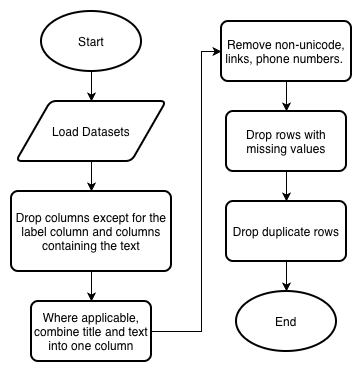
\includegraphics[width=0.5\linewidth]{FYP_Research_Methodology.png}
    \caption{Figure depicts preprocessing steps in flowchart form}
    \label{fig:preprcessing_flowchart}
\end{figure}

After the above processes, the data was tokenised using BERT's tokeniser without further processing steps.

\subsection{Experimental Setup}
For BERT, fine-tuning was done on a base BERT-uncased model into a 2-label classification model. A similar process was done for TPA-BERT, the proposed model, with the addition of adversarial training steps.

All training was done with 5-fold cross-validation, with an initial split of 85\% train and 15\% test (held on for the final evaluation of each fold). The 85\% train is split again later on into 80\% train and 20\% validation for each fold. All splits were stratified. For cross-dataset evaluation, only the best fold by validation F1-score is evaluated. 

\section{Results}

Results for model performance is the mean of all fold's test set evaluation. For conciseness, validation F1-scores and standard deviation are not reported due to the differences being rather insignificant. Note that for cross-dataset evaluation, only the results for the model trained on WELFake is reported on.

\begingroup
\setlength{\tabcolsep}{3pt}
\renewcommand{\arraystretch}{1.3}
\setlength\LTleft{0pt}
\setlength\LTright{0pt}
\begin{longtable}{@{} l c c c c @{}}
\caption{Baseline BERT Results} \label{tab:bert_results} \\
\toprule
\textbf{Dataset Name} & \textbf{Accuracy} & \textbf{Precision} & \textbf{Recall} & \textbf{F1} \\
\midrule
\endfirsthead

\multicolumn{5}{c}{{\bfseries \tablename\ \thetable{} (continued)}} \\
\toprule
\textbf{Dataset Name} & \textbf{Accuracy} & \textbf{Precision} & \textbf{Recall} & \textbf{F1} \\
\midrule
\endhead

\bottomrule
\multicolumn{5}{r}{{Continued on next page}} \\
\endfoot

\bottomrule
\endlastfoot
WELFake & 0.9917 & 0.9920 & 0.9897 & 0.9908 \\
FakeNewsNet & 0.8497 & 0.8768 & 0.9325 & 0.9037 \\
Fake News Detection & 0.9976 & 0.9986 & 0.9971 & 0.9978 \\
ISOT & 0.9996 & 0.9991 & 1.0000 & 0.9995 \\
Fake News Classification & 0.9934 & 0.9948 & 0.9929 & 0.9938 \\
\end{longtable}
\endgroup

The results from the fine-tuned BERT models exhibited very high accuracy, recall and precision. As can be referred to in Table \ref{tab:bert_results}, it appears that the FakeNewsNet dataset was the most challenging dataset. All the other datasets proved to be no challenge for each of their fine-tuned BERT models. It is however notable that the F1-scores are in the range (with the exception of the FakeNewsNet dataset) exceed 0.99 which is very high, this may indicate that these datasets may have gathered the data for their positive and negative classes with a methodology that unknowingly introduced some level of data leakage. The alternative is that BERT is simply a very effective model, but the relatively lower performance of BERT on the FakeNewsNet dataset indicates the other datasets may be of lower quality or are less challenging. 

However, it must be noted that FakeNewsNet differs from the other datasets as it has a significant class imbalance, with about 75\% of the records belonging to the positive class. Furthermore, FakeNewsNet only contains the title of the article, and does not contain the main article body. For these reasons, FakeNewsNet presents a unique challenge which may explain the relatively (compared to other datasets) poor performance of BERT.

\begingroup
\setlength{\tabcolsep}{3pt}
\renewcommand{\arraystretch}{1.3}
\setlength\LTleft{0pt}
\setlength\LTright{0pt}
\begin{longtable}{@{} l c c c c @{}}
\caption{Cross Dataset Generalisation (BERT) - WELFake Only} \label{tab:bert_cross_results} \\
\toprule
\textbf{Dataset Name} & \textbf{Accuracy} & \textbf{Precision} & \textbf{Recall} & \textbf{F1} \\
\midrule
\endfirsthead

\multicolumn{5}{c}{{\bfseries \tablename\ \thetable{} (continued)}} \\
\toprule
\textbf{Dataset Name} & \textbf{Accuracy} & \textbf{Precision} & \textbf{Recall} & \textbf{F1} \\
\midrule
\endhead

\bottomrule
\multicolumn{5}{r}{{Continued on next page}} \\
\endfoot

\bottomrule
\endlastfoot
FakeNewsNet & 0.6984 & 0.7562 & 0.8872 & 0.8165 \\
Fake News Detection & 0.2231 & 0.3302 & 0.4054 & 0.3640 \\
ISOT & 0.9992 & 0.9998 & 0.9983 & 0.9991 \\
Fake News Classification & 0.0188 & 0.0380 & 0.0336 & 0.0357 \\
\end{longtable}
\endgroup

The best fold by validation f1-score was selected for cross dataset evaluation. 

The results show that the model trained on WELFake performed quite well for FakeNewsNet and ISOT, and much poorer for Fake News Detection and Fake News Classification datasets. The model most likely performed better on the FakeNewsNet and ISOT datsets due to the similarities between WELFake and the aforementioned datasets. WELFake contains the article title (originally in its own column; appended at the beginning with the rest of the text during preprocessing) which may be why it performs well on the FakeNewsNet dataset. As for ISOT, it may be that these two datasets are very similar, and as a result the model was able to generalise well for ISOT. 

As for the other two datasets: Fake News Detection and Fake News Classification, these datasets likely performed poorly due to being too different than WELFake. As a result the model was unable to generalise for these models thus causing the poor results. This is despite both datsets having 'title' columns initially. This may be because they also contained a 'text' column, which contained the rest of the article; this is in contrast to FakeNewsNet, which contained only the 'title' column. This addition of more detail may have increased the differences between the WELFake and Fake News Detection and Fake News Classification datasets. Furthermore, the methodology for collecting these datasets may have been substantially different than the methodology used to collect the WELFake dataset, causing the datasets to differ substantially. These factors could have confused the model, preventing it from effectively generalising.

\begingroup
\setlength{\tabcolsep}{3pt}
\renewcommand{\arraystretch}{1.3}
\setlength\LTleft{0pt}
\setlength\LTright{0pt}
\begin{longtable}{@{} l c c c c @{}}
\caption{TPA-BERT Results} \label{tab:tpa_bert_results} \\
\toprule
\textbf{Dataset Name} & \textbf{Accuracy} & \textbf{Precision} & \textbf{Recall} & \textbf{F1} \\
\midrule
\endfirsthead

\multicolumn{5}{c}{{\bfseries \tablename\ \thetable{} (continued)}} \\
\toprule
\textbf{Dataset Name} & \textbf{Accuracy} & \textbf{Precision} & \textbf{Recall} & \textbf{F1} \\
\midrule
\endhead

\bottomrule
\multicolumn{5}{r}{{Continued on next page}} \\
\endfoot

\bottomrule
\endlastfoot
WELFake & 0.9882 & 0.9852 & 0.9888 & 0.9870 \\
FakeNewsNet & 0.8425 & 0.8702 & 0.9305 & 0.8994 \\
Fake News Detection & 0.9947 & 0.9933 & 0.9971 & 0.9952 \\
ISOT & 0.9993 & 0.9987 & 0.9998 & 0.9993 \\
Fake News Classification & 0.9890 & 0.9938 & 0.9858 & 0.9898 \\
\end{longtable}
\endgroup

The results for TPA-BERT were excellent, with results exceeding F1-scores of 0.95 with the exception of FakeNewsNet. When comparing the results against BERT, BERT very slightly (<0.005 difference in f1 score) outperforms TPA-BERT, but this is not a significant difference and could have been caused by chance. Overall these results followed the same pattern as BERT, with all datasets doing exceptionally with the exception of FakeNewsNet.

\begingroup
\setlength{\tabcolsep}{3pt}
\renewcommand{\arraystretch}{1.3}
\setlength\LTleft{0pt}
\setlength\LTright{0pt}
\begin{longtable}{@{} l c c c c @{}}
\caption{Cross Dataset Generalisation (TPA-BERT) - WELFake Only} \label{tab:tpa_bert_cross_results} \\
\toprule
\textbf{Dataset Name} & \textbf{Accuracy} & \textbf{Precision} & \textbf{Recall} & \textbf{F1} \\
\midrule
\endfirsthead

\multicolumn{5}{c}{{\bfseries \tablename\ \thetable{} (continued)}} \\
\toprule
\textbf{Dataset Name} & \textbf{Accuracy} & \textbf{Precision} & \textbf{Recall} & \textbf{F1} \\
\midrule
\endhead

\bottomrule
\multicolumn{5}{r}{{Continued on next page}} \\
\endfoot

\bottomrule
\endlastfoot
FakeNewsNet & 0.6996 & 0.7520 & 0.8995 & 0.8191 \\
Fake News Detection & 0.2178 & 0.3246 & 0.3946 & 0.3562 \\
ISOT & 0.9982 & 0.9994 & 0.9968 & 0.9981 \\
Fake News Classification & 0.0196 & 0.0383 & 0.0338 & 0.0359 \\
\end{longtable}
\endgroup

The cross-dataset evaluation for TPA-BERT followed the same pattern as observed in the BERT results, with FakeNewsNet and ISOT performing better in comparison to the rather abysmal performance on the other two datasets. The results however, when compared against BERT were only slightly better (<0.008 difference in f1 score), this small difference may be attributed to randomness and is likely not sigificant. These results indicate that the adversarial technique used in TPA-BERT failed to generalise the model sigificantly. 

There could be several causes for this: lack of depth to the text perturbation technique, use of the CLS token, and the fact these perturbations are not 'natural'. The text perturbation techniques employed were: synonym substitution, random swapping and random deletion. These techniques most likely were unable to meaningfully change the overall semantic meaning of the textual input. This flows directly to the next point, use of the CLS token: the CLS token, as previously mentioned is a 768 dimensional representation of the input text (essentially a semantic summary of the input text). This CLS token makes the order of the text less relevant, as the classifier only uses this CLS token. This means that without genuine semantic variation, the adversarial training only taught the model how to 'autocorrect' the perturbations in the text.

Lastly, the perturbations do not produce meaningful variations. The random synonym substitution, swapping and deletion creates text which is not a meaningful variation of human writing. This means that while the model learned to adapt to the perturbations, it didn't learn to actually handle genuine variations in human writing styles. Had there been geuine variations, the semantics may have changed as well, allowing the adversarial training to force the model to identify variation-agnostic features while preserving the ability of the model to detect styles indicative of fake news; essentially teaching the models to classify the 'fakeness' of news based on less superficial features.

However, even if the issues mentioned above were rectified, it is unlikely to produce a practical generalised model. Real world data and the datasets available continue to have substantial differences. This is exacerbated by the impossibility of knowing the ground truth of all the data in the wild. Nonetheless, this research has proven that current approaches to fake news detection are more than capable of performing well when working with a dataset. However, the actual process of generalising a model to a degree where it can be reliably in real-world settings remains elusive. Although there are likely more successful attempts than the one described here like by \textcite{BERT-finetuning}, there remains significant work to be done in regards to generalisation. 

\section{Conclusion}
There is no significant difference in performance between BERT and TPA-BERT. This indicates that the perturbation techniques applied on the training datasets failed to cause TPA-BERT's adversarial training to increase the generalisation of the model. Further reasoning was thoroughly discussed in the previous section. 

Many things could be improved upon in further work, from different perturbation strategies, use of BERT variations, BERT-layer freezing and hyperparamtere optimisation. Firstly, future work could attempt perturbations at a deeper level, such as by perturbing the embedding level for example. Or attempt to perturb the dataset to produce human-like variations in the data. Secondly, this research only utilised the BERT model, future work could attempt to work with BERT variations such as RoBERTa. Furthermore, during the literature review a technique involving the freezing of layers in BERT was used by \textcite{BERT-finetuning}, which produced some level of improvement in regards to optimisation. Future work could employ BERT layer-freezing to improve generalisation. And lastly, hyperparamter optimisation was not conducted, further research could have a hyperparameter optimisation step to improve model performance.

Additionally this research suffered from computational resource limitations. This impacted decisions related to batch size, epochs and token cap and contributed to the decision not to conduct hyperparameter optimisation. 

In concluion, this research has demonstrated that while BERT can perform very well on the datasets it is trained on, BERT doesn't generalise very well. Furthermore generalisation performance likely depends on similarity between the dataset used to train a model and the dataset being tested. And lastly, he experiments with the proposed model, TPA-BERT, showed that adversarial training on a perturbed dataset failed to increase generalisation compared to BERT. 

\printbibliography



\end{document}
